\documentclass{article}
\usepackage{amsmath}
\usepackage{graphicx}
\providecommand{\brak}[1]{\ensuremath{\left(#1\right)}}

\begin{document}
\title{Maths Assignment}
\author{Karyampudi Meghana Sai\\ EE23BTECH11031}
\maketitle

\section*{Problem Statement}
Write the first five terms of the sequence \(a_n = \frac{n(n^2+5)}{4}\).

\section*{Solution}
The relation between \(x(n)\) and \(u(n)\):
\begin{align}
 x(n) &= \left(\frac{(n+1)^3+5(n+1)}{4}\right) u(n)\label{eq:1}
\end{align}
Z-transform of \(n^ku(k)\) in terms of the \(k\)-th derivative of \(U(z)\):
\begin{align}
n^k u(n) &\overset{\text{ZT}}{\longleftrightarrow} (-1)^k z^k \frac{d^k}{dz^k}U(z)
\end{align}

\begin{align}
    \mathcal{Z}\{nu(n)\} &= \frac{z^{-1}}{\brak{1 - z^{-1}}^2}\label{eq:3} \text{ [ROC: } \lvert z \rvert > 1\text{]} \\
    \mathcal{Z}\{n^2u(n)\} &= \frac{\brak{z^{-1}}(1+\brak{z^{-1}})}{\brak{1 - z^{-1}}^3}\label{eq:4} \text{ [ROC: } \lvert z \rvert > 1\text{]} \\
    \mathcal{Z}\{n^3u(n)\} &= \frac{\brak{z^{-1}}\brak{1+4z^{-1}+z^{-2}}}{\brak{1 - z^{-1}}^4}\label{eq:5} \text{ [ROC: } \lvert z \rvert > 1\text{]}
\end{align}
Referencing the equations \eqref{eq:3}, \eqref{eq:4}, and \eqref{eq:5}.
\begin{equation}
\mathcal{X}\{z\} = \frac{\brak{z^{-1}}(1+4z^{-1}+z^{-2})}{4\brak{1-z^{-1}}^4} + \frac{3\brak{z^{-1}}(1+z^{-1})}{4\brak{1-z^{-1}}^3} + \frac{2z^{-1}}{\brak{1 - z^{-1}}^2} + \frac{3}{2\brak{1- z^{-1}}} \text{ [ROC: } \lvert z \rvert > 1\text{]}
\end{equation}

\newpage
\begin{figure}
    \centering
    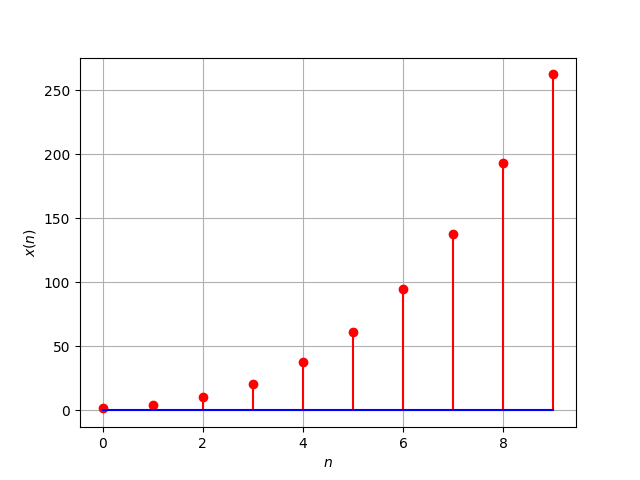
\includegraphics{figs/plot.png}
    \caption{Plot of equation \eqref{eq:1}\label{fig:plot}}
\end{figure}

\end{document}

